\documentclass[12pt]{article}
\usepackage[paper=a4paper,dvips,top=2.5cm,left=2.5cm,right=2.5cm,
    foot=2cm,bottom=2.5cm]{geometry}
\usepackage[utf8]{inputenc}
\usepackage{lipsum}
\usepackage{graphicx}
\usepackage{caption}
\usepackage{subcaption}
\usepackage{amsmath}
\usepackage{gensymb}

\begin{document}
\setlipsumdefault{1-10}
% %%%%%%%%%%%%%%%%%%%%%%%%%%%%%%%%%%%%%%%%%%%%%%%%%%%%%%%%%%%%%%%
% %%%%%%%%%%%%%%%%%%%%%REMERCIEMENTS
% %%%%%%%%%%%%%%%%%%%%%%%%%%%%%%%%%%%%%%%%%%%%%%%%%%%%%%%%%%%%%%%
% \part*{Remerciement}
% Je remercie....
% \pagebreak
% %%%%%%%%%%%%%%%%%%%%%%%%%%%%%%%%%%%%%%%%%%%%%%%%%%%%%%%%%%%%%%%
% %%%%%%%%%%%%%%%%%%%%%ENTREPRISE
% %%%%%%%%%%%%%%%%%%%%%%%%%%%%%%%%%%%%%%%%%%%%%%%%%%%%%%%%%%%%%%%
% \part*{Entreprise}
% Thales...
% \pagebreak
% %%%%%%%%%%%%%%%%%%%%%%%%%%%%%%%%%%%%%%%%%%%%%%%%%%%%%%%%%%%%%%%
% %%%%%%%%%%%%%%%%%%%%%INTRO
% %%%%%%%%%%%%%%%%%%%%%%%%%%%%%%%%%%%%%%%%%%%%%%%%%%%%%%%%%%%%%%%
% \part*{Introduction}
% Contexte
% -au sein de l'entreprise
% -au sein de l'equipe
% -au sein du domaine technique
% But du stage
% -resultats attendus
% -precedents resultats dans le domaine
% \pagebreak
% \part*{Deroulement}
% \section{Contrôle caméra et flux vidéo}

% \pagebreak
\section{Détection de personne}
Afin de mettre en place un suivi efficace des personnes, il faut commencer par être capable de détecter ces personnes. Il a donc fallu en premier lieu décider d'une méthode de détection de personnes adaptée à notre application. De nombreuses méthodes différentes existent dans ce domaine, mais l'environnement dans lequel nous effectuons cette détection fixe nos besoins:\\
\\
-le suivi des personnes devant être fait en temps réel, il nous faut un algorithme suffisamment rapide pour ne pas avoir un impact trop important sur les performances du système complet;\\
-le fait que nous travaillons avec un caméra PTZ et que ce travail soit destiné à fonctionner dans des environnements variés élimine les méthodes de détection se basant sur un fond connu.\\
\\
Mon choix s'est porté sur une détection basée sur les histogramme de gradient orienté (HOG) pour son efficacité reconnue, sa rapidité et le fait que cet algorithme est suffisamment populaire pour pouvoir trouver des implémentations simples et des classifieurs entrainés sur des jeu de données correspondants à notre cas de figure.\\
L’implémentation utilisée est celle présente dans OpenCV sous le nom de ``HOGDescriptor'' associé à un classifieur de type machines à vecteurs de support (SVM). Le descripteur utilisé est celui par défaut d'OpenCV pour les personnes.
\subsection{Principe de la détection HOG}
Cette méthode a été présentée par Navneet Dalal et Bill Triggs en 2005 dans le papier ``Histograms of Oriented Gradients for Human Detection''.
Elle consiste en une série d'étapes illustrées dans la figure~\ref{fig:hog_topo}.
\begin{figure}[!ht]
    \centering
	    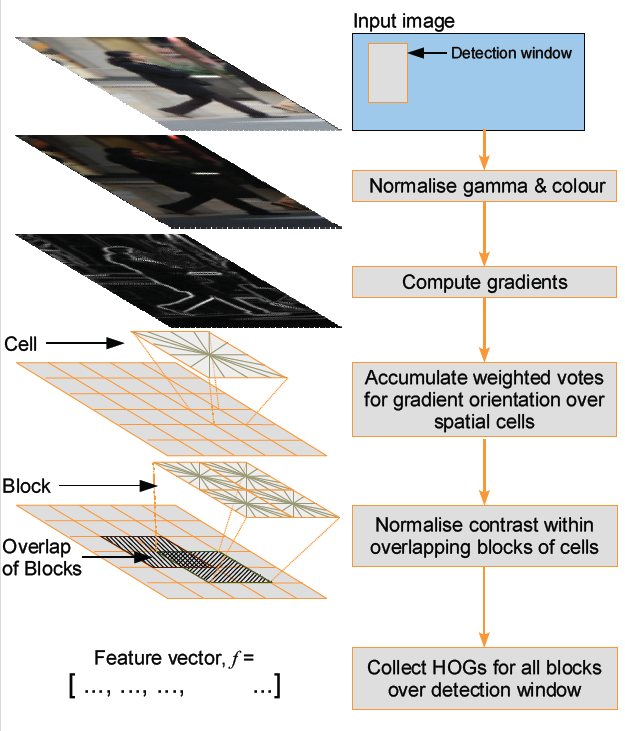
\includegraphics[width=0.4\textwidth]{img/hog_topo.png}
	    \caption{Illustration HOG+SVM}
   	    \label{fig:hog_topo}
\end{figure}

%%%%%%%%%%%%%%%%%%%%%%%%%%
\subsection{Descripteur HOG}
Dans cette méthode, le descripteur (nommé HOG-D) est basé sur un ensemble d'histogrammes de gradient orientés. Les différentes étapes nécessaires au calcul de ces histogrammes est décris ci-dessous:
\subsubsection{Découpage de l'image}
Le descripteur est calculé pour une image de 64x128 pixels, ces dimensions représentent les proportions choisi pour une personne. C'est également la résolution utilisée pour la base d'image ``INRIA Person Dataset'' réunie pour tester cette méthode.\\
Cette image est découpée en cellules de 8x8 pixels, ces cellules sont utilisées pour faire des blocs de 2x2 cellules (16x16 pixels). Les blocs se recoupent à 50\%, ce qui donne un total de 7 blocs en largeur par 15 blocs en hauteur.\\
On a donc au final un total de 105 blocs contenant chacun 4 cellules de 8x8 pixels.
\begin{figure}[!ht]
\centering
\begin{subfigure}{.3\textwidth}
  \centering
  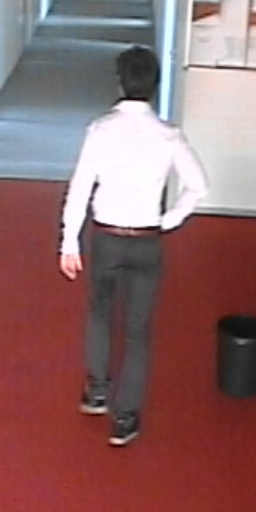
\includegraphics[width=.5\linewidth]{img/person.png}
  \caption{Image d'origine}
  \label{fig:kernel_sx}
\end{subfigure}%
\begin{subfigure}{.3\textwidth}
  \centering
  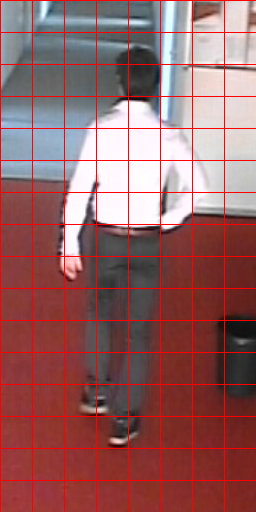
\includegraphics[width=.5\linewidth]{img/cell.png}
  \caption{Découpage en cellules}
  \label{fig:kernel_sy}
\end{subfigure}
\begin{subfigure}{.3\textwidth}
  \centering
  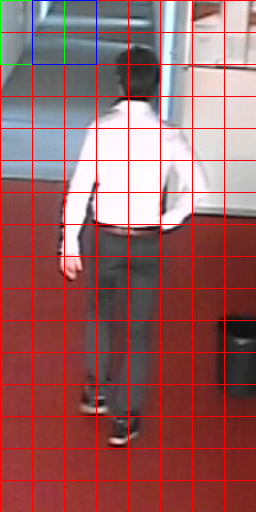
\includegraphics[width=.5\linewidth]{img/block.png}
  \caption{Deux premiers blocs}
  \label{fig:kernel_sy}
\end{subfigure}
\caption{Découpage de l'image en blocs et en cellules}
\label{fig:kernels}
\end{figure}
\subsubsection{Calcul des gradients}
Les gradients orientés sont calculés à l'aide de deux gradients pour chaque pixel: un gradient horizontal et un gradient vertical notés $S_{x}$ et $S_{y}$ tel que:
\[S_{x(i,j)}=I_{(i+1,j)}-I_{(i-1,j)}\]
\[S_{y(i,j)}=I_{(i,j+1)}-I_{(i,j-1)}\]
Les noyaux utilisés pour calculer ces deux valeurs sont illustrés dans la fig ???
\begin{figure}[!ht]
\centering
\begin{subfigure}{.3\textwidth}
  \centering
  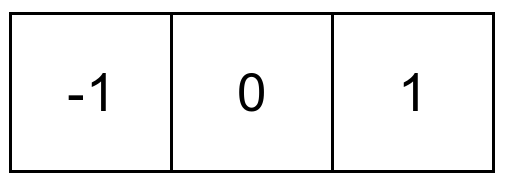
\includegraphics[width=.45\linewidth]{img/Sx.png}
  \caption{$Sx$}
  \label{fig:kernel_sx}
\end{subfigure}
\begin{subfigure}{.3\textwidth}
  \centering
  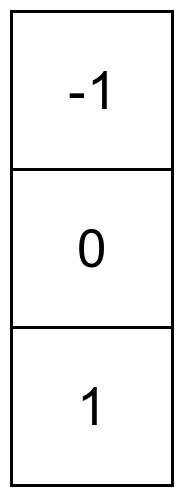
\includegraphics[width=.15\linewidth]{img/Sy.png}
  \caption{$Sy$}
  \label{fig:kernel_sy}
\end{subfigure}
\caption{Noyaux des gradients horizontaux (a) et verticaux (b)}
\label{fig:kernels}
\end{figure}
Blabla le gradient orienté est représenté par le vecteur: 
$\bar{S}=\begin{pmatrix}S_{x}\\S_{y}\end{pmatrix}$
Les caractéristiques du gradient sont donc:
\[\bar{S}:\begin{cases}
\|S\|=\sqrt{S_{x}^{~2}+S_{y}^{~2}}\\
\Omega_{S} = arctan(\frac{S_{y}}{S_{x}})
\end{cases}\]
\subsubsection{Calcul des histogrammes}
Pour chaque cellule, un histogramme est obtenue grâce à la somme pondérée des orientations des gradients. Cet histogramme est réalisé pour 9 valeurs d'orientation par pas de 20\degree les orientations vont donc de 0\degree~à 180\degree.
\begin{figure}[!ht]
    \label{fig:orientations}
    \centering
	    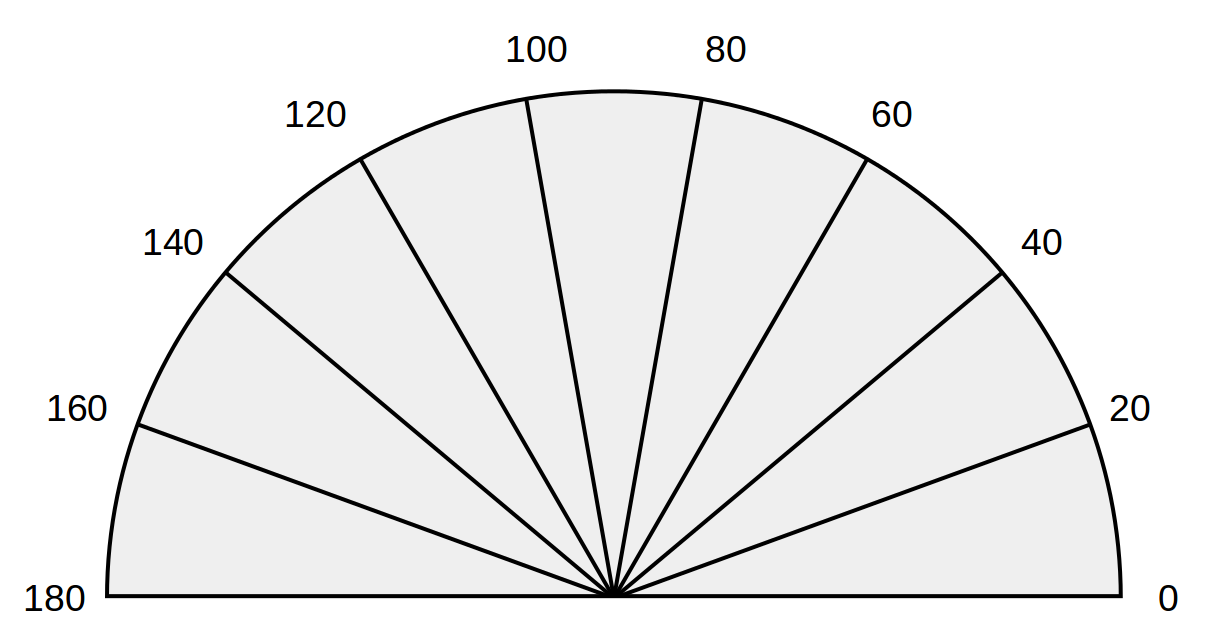
\includegraphics[width=0.5\textwidth]{img/angles.png}
	    \caption{Découpage des orientations des gradients en 9 sections}
\end{figure}
Les centres de ces intervalles sont donc [10;30;50;70;90;110;130;150;170]\degree.
\begin{figure}[!ht]
    \label{fig:histo}
    \centering
	    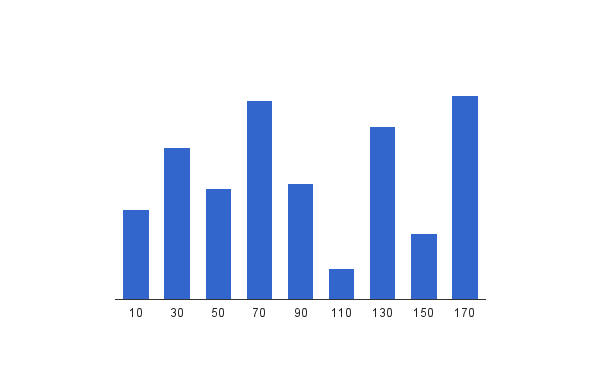
\includegraphics[width=0.5\textwidth]{img/histo.png}
	    \caption{Histogramme obtenu avec centres des intervalles}
\end{figure}
Un gradient ayant pour orientation 50\degree~verra donc son poids (sa norme) ajouté à la barre [40;60]\degree~de l'histogramme de sa cellule.
Les gradients dont l'orientation se situe entre deux centres d'intervalles ont leur poids repartis entre les deux segments de l'histogramme par un principe d'interpolation trilinéaire.\\
\\
Ainsi, si on prend un gradient $\bar{X}$, de norme $\|X\|$ et d'orientation $\theta_{X}=55\degree$, son poids ($\|X\|$) sera reparti entre les segments [40;60]\degree~et [60;80]\degree~de l'histogramme ayant pour centres 50\degree~et 70\degree~respectivement.
Si on note les poids assignés aux deux segments $P_{X50}$ et $P_{X70}$, on obtient:
\[
\begin{cases}
P_{50}(X)=\left ( 1-\frac{|\theta_{X}-50|}{20} \right )*\|X\| = \frac{3}{4}*\|X\|\\
P_{70}(X)=\left ( 1-\frac{|\theta_{X}-70|}{20} \right )*\|X\| = \frac{1}{4}*\|X\|
\end{cases}
\]
Cela permet d'éviter qu'un gradient avec une norme importante se situant à la limite entre deux sections de l'histogramme puisse faire varier le résultat de manière trop importante.
\subsubsection{Concaténation et normalisation}
Une fois les histogrammes des quatre cellules d'un bloc calculés, ils sont concaténés afin de former un vecteur de 36 valeurs (4*9).\\
\\
Afin de diminuer l'impact des variations de contraste locales, les histogrammes des blocs sont tous normalisé en divisant leurs valeurs par la norme du vecteur obtenue. On a ainsi un descripteur invariant par rapport au contraste local (bloc de 32x32 pixels) ainsi que par rapport à la luminosité de l'image (caractéristique inhérente aux gradients).
Une fois les histogrammes des blocs sont à leur tour concaténés pour obtenir l'histogramme final.\\
\\
Le descripteur HOG-D nous donne donc vecteur de 3780 valeurs (105 blocs * 36 valeurs) pour représenter une image de 128x64 pixels.
%%%%%%%%%%%%%%%%%%%%%%%%%%

\subsection{Classifieur}
Ce descripteur va être utilisé avec un classifieur afin d'effectuer notre détection de personne. Le classifieur utilisé ici est le même que celui utilisé par Dalal et Bill Triggs, une machine à vecteurs de support linéaire (\textit{linear SVM}) entrainée à l'aide de \textit{SVMLight}.\\
\\
\subsubsection{Classification}
Le principe d'un classifieur linéaire est, à l'aide d’exemples positifs et négatifs, de déterminer un hyperplan permettant de séparer l'espace des positifs et celui des négatifs. Un exemple d'ensemble de points positifs et négatifs dans un espace en deux dimensions est présenté en figure~\ref{fig:trainingexamples}.
\begin{figure}[!ht]
    \centering
	    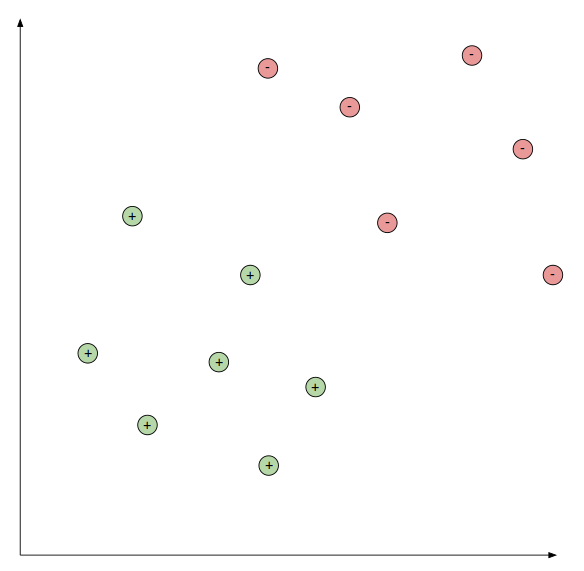
\includegraphics[width=0.4\textwidth]{img/trainingexamples.png}
	    \caption{Exemples positifs et négatifs utilisés pour entrainer la SVM dans un espace 2D}
        \label{fig:trainingexamples}
\end{figure}
La particularité de la SVM est d'avoir pour but de trouver l'hyperplan le plus distant des exemples négatifs et positifs. C'est le principe de la route la plus large, on cherche à trouver la route la plus large pouvant séparer les exemples, et une fois définie, l'hyperplan choisi est au centre de la ``route''.\\
Ce principe est illustré dans les figures~\ref{fig:multipleplans} et~\ref{fig:wideststreet}.
\begin{figure}[!ht]
\centering
\begin{minipage}{.5\textwidth}
  \centering
  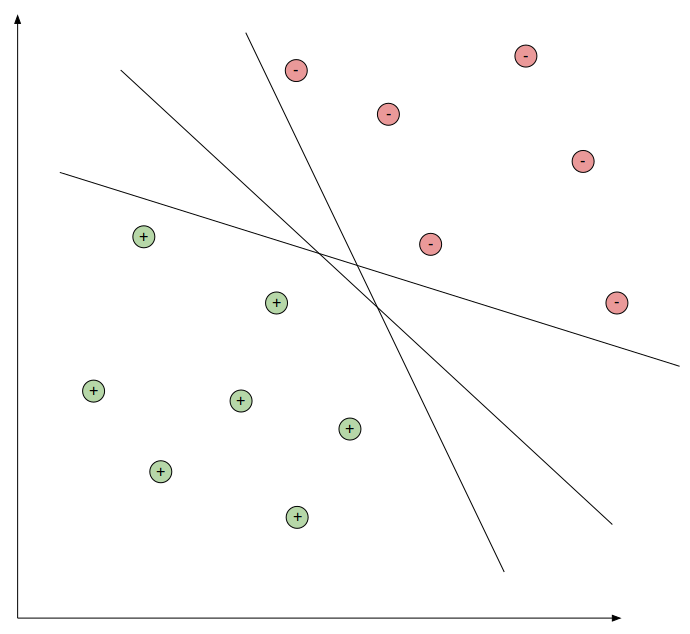
\includegraphics[width=.8\linewidth]{img/multipleplans.png}
  \captionof{figure}{Différents hyperplans valides}
  \label{fig:multipleplans}
\end{minipage}%
\begin{minipage}{.5\textwidth}
  \centering
  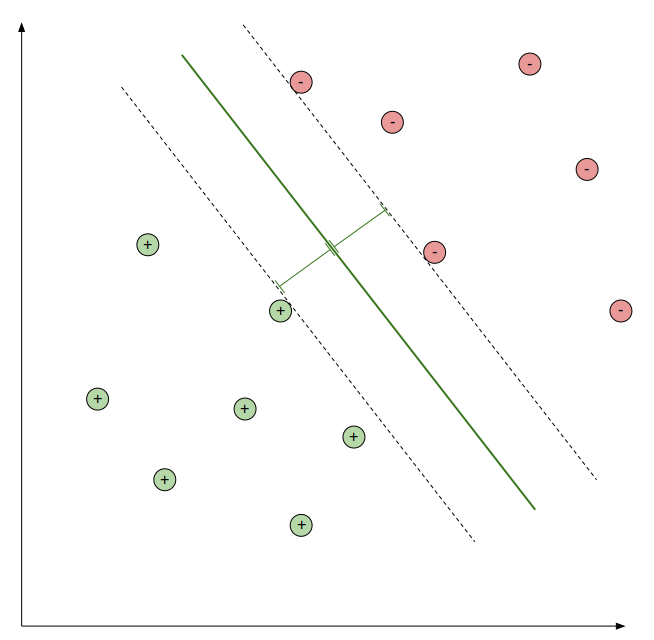
\includegraphics[width=.8\linewidth]{img/wideststreet.png}
  \captionof{figure}{Hyperplan avec la marge la plus large}
  \label{fig:wideststreet}
\end{minipage}
\end{figure}
\\
\\
Une fois l'hyperplan défini lors de l'entrainement de la SVM avec des exemples positifs et négatifs, on peut s'en servir pour déterminer si un point donné dans cet espace est positif ou non selon sa position par rapport à l'hyperplan.\\
Pour cela, on utilise un vecteur unitaire normal à l'hyperplan sur lequel on projette le vecteur des paramètre du point expérimental, la valeur de cette projection est comparée avec celle déterminée par l'hyperplan.\\\\
Si on note la distance entre l'origine et l'hyperplan $C$, $\bar{w}$ le vecteur unitaire normal à l'hyperplan, et $\bar{X}$ le point expérimental à classifier, on a la relation suivante:
\[\alpha=\bar{X}\cdot\bar{u}~
\begin{cases}
\alpha\geq C\rightarrow~$cas positif$\\
\alpha<C\rightarrow~$cas négatif$
\end{cases}
\]
\begin{figure}[!ht]
    \centering
	    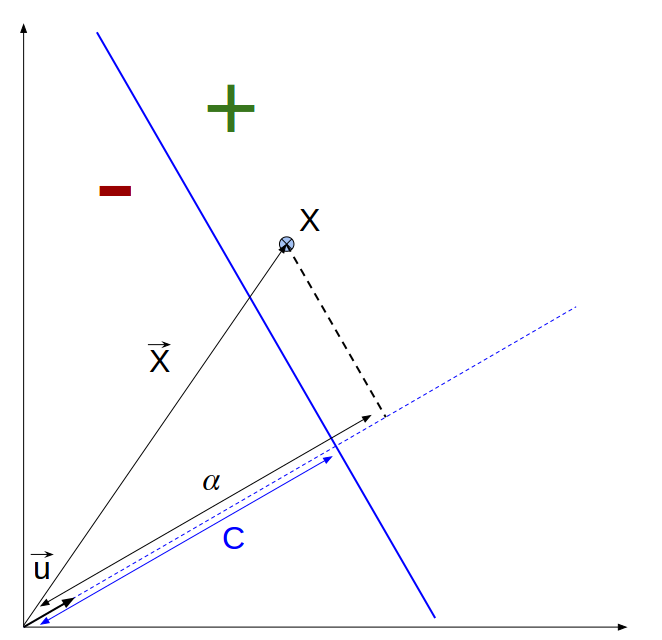
\includegraphics[width=0.4\textwidth]{img/projection.png}
	    \caption{Utilisation de l'hyperplan pour classifier un exemple X}
        \label{fig:projection}
\end{figure}
\subsubsection{Fenêtre glissante multi-échelle et suppression des non-maxima}
Une fois la SVM entrainée, on peut utiliser une fenêtre glissante le long d'une image afin de déterminer les parties de l'images classifiées comme des personnes. Pour pouvoir détecter les personnes de différentes tailles et à différentes distances on repasse la fenêtre à différentes échelles.\\
\\
On a alors une liste des sous-rectangles de l'images contenant une personne, le problème étant qu'une même personne peut être détectée dans plusieurs rectangles de tailles et de positions légèrement différentes et on obtient une multitudes de rectangles positifs pour une seule personne.\\
Afin de résoudre ce problème, on utilise un algorithme de suppression des non-maxima sur l'ensemble des rectangles obtenus.\\\\
Le principe est de mesurer la similitude entre deux rectangle, notée $\epsilon$, en fonction de leurs tailles et positions, au delà d'un certain seuil paramétrable, les deux rectangles similaires sont réunis.\\
On peut également choisir un seuil pour le nombre minimum de rectangles dans un cluster pour que la détection soit gardée, et enfin tout les rectangles étant inclus dans des rectangles plus grand avec plus d’occurrences sont également supprimés.\\
Le résultat cet algorithme une fois paramétré est illustré dans la figure~\ref{fig:nonmaxima}.
\begin{figure}[!ht]
	\centering
	\begin{subfigure}{.45\textwidth}
		\centering
		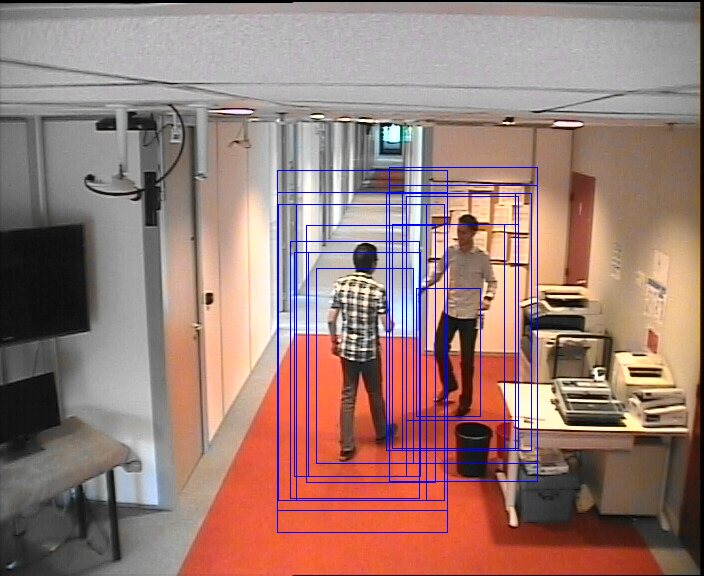
\includegraphics[clip=true,trim=200 0 100 100,width=\linewidth]{img/nonmax1.png}
		\caption{Résultat de HOG-D+SVM linéaire}
	\end{subfigure}
	\begin{subfigure}{.45\textwidth}
		\centering
		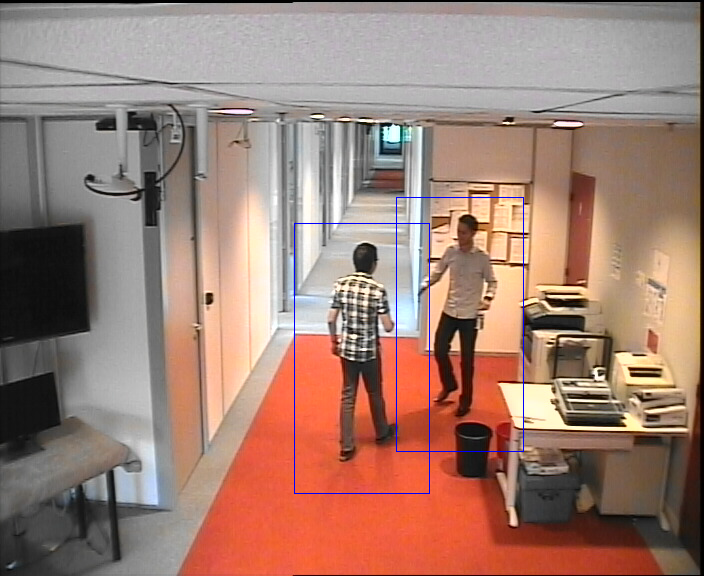
\includegraphics[clip=true,trim=200 0 100 100,width=\linewidth]{img/nonmax2.png}
		\caption{Suppression des non-maxima}
	\end{subfigure}
	\caption{Algorithme de suppression des non-maxima}
	\label{fig:nonmaxima}
\end{figure}

\subsection{Resultat obtenues}
-10FPS
-pratiquement aucun faux positifs
(géré par le tracking sisi)
-pratiquement complet niveau detection face/dos
(géré aussi maggle)
-lacune: detection de profil

% \section{Suivi de personnes}
% \section{Decision de flight plan de caméra}
% \section{Detection de visage}
% \pagebreak
% \part*{Resultats et amélioration}
% \pagebreak
% \part*{Conclusion}
% \pagebreak

\end{document}